Simulation is a fast and cheap way of testing drone control algorithms, as it cuts out the overhead of physical components and the risk of fatal, expensive crashes. However, it does have the added overhead of adapting a specific model to a specific simulation environment, which can be a daunting task. Furthermore, the results of the simulation - particularly the model physics - likely will not translate directly to the real world. Ultimately this means that simulation can be aptly used for testing the landing system at a high level, but that transitioning to real world flight will involve incremental re-testing. In other words, simulation is only a good first step.


\subsection{Setup and Tools}
\label{subsection:setup_and_tools}

The Gazebo 9 simulator and the ArduPilot-compatible Iris quadcopter drone model (and included gimbal model) are provided in the open source community, as discussed in Section \ref{subsection:gazebo} and Section \ref{subsection:ardupilot_gazebo} respectively. These systems have existing integration with each other and with \gls{ROS}, making them an ideal combination of tools for this project. The development of a new drone model for simulation is beyond the scope of this project. However, even though there is a slight discrepancy in that the simulation model is a quadcopter and the destination platform is a hexacopter, the proposed landing system is abstracted enough to overcome this difference. All of the commands sent by the landing controller are target velocities rather than primitive controls such as throttle signals to specific motors. The frame (quadcopter or hexacopter) can be manually set in the ArduPilot on-board firmware.

% The open-source autopilot softwares ArduPilot and PX4 both have open source drone models available for use in an open source simulator called Gazebo. The model that has been used in this simulation is Gazebo's Iris quadcopter, which has plugins for both ArduPilot and PX4. 

\subsubsection{Simulation World}

\begin{figure}[ht]
    \centering
    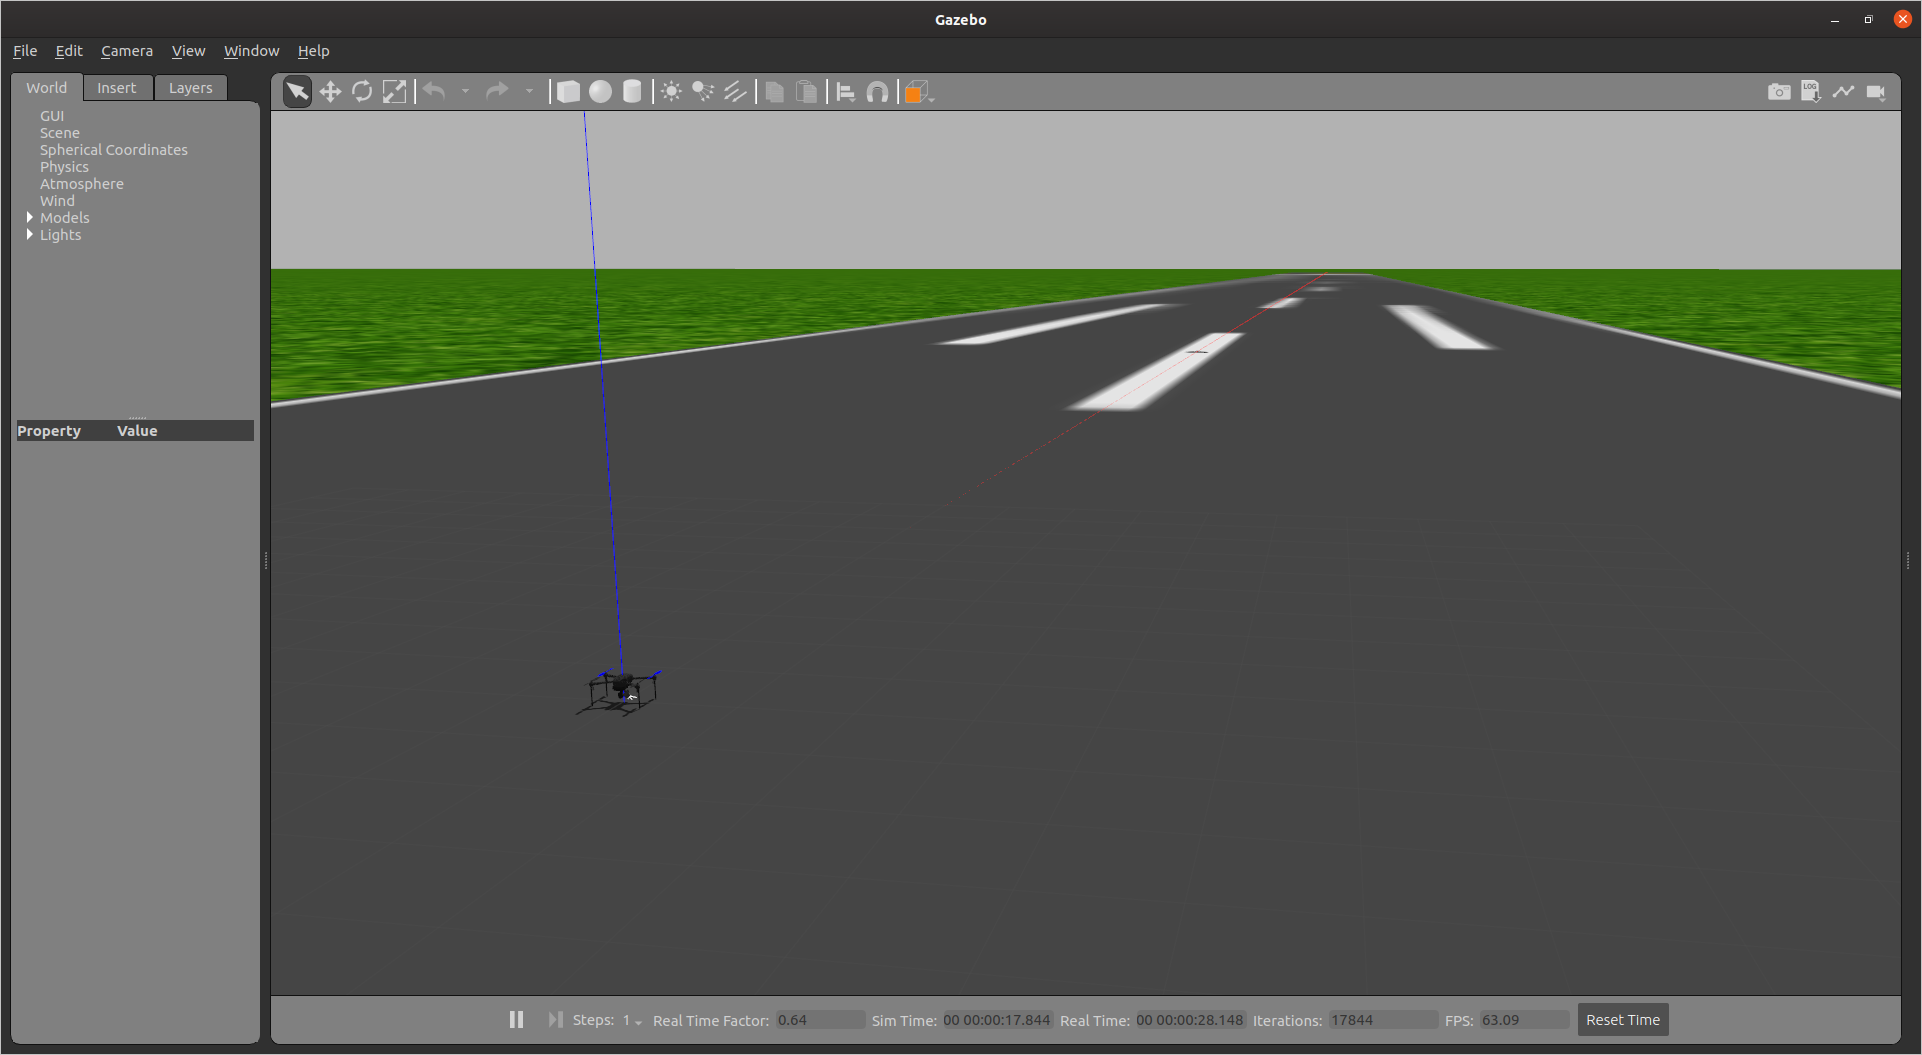
\includegraphics[width=0.6\textwidth]{images/gazebo.png}
    \caption{Gazebo GUI with the Iris quadcopter model.}
    \label{fig:gazebo}
\end{figure}

% \subsubsection{Simulation World}

The simulation uses Gazebo 9 as its base, as shown in Figure \ref{fig:gazebo}. However, in order to interface with ROS, Gazebo is launched through ROS itself, with the following command: \texttt{roslaunch gazebo\_ros sandbox.launch}, where \texttt{sandbox.launch} opens a ``sandbox'' world created for the purpose of experimentation. It is an edited version of the \texttt{iris\_ardupilot.world} which includes a landing platform made from fiducial markers, explained in Section \ref{subsection:landing_pad_design}. It includes the specification for the Iris quadcopter, along with an edited version of the Iris' gimbal. The edited version of the gimbal adds a weightless, simulated camera sensor that provides its detected image to an instance of ROS as a ROS topic. This particular sensor is available from the \texttt{gazebo\_ros\_pkgs} repository. This is necessary because the included gimbal model does not include a camera sensor. The typical paradigm for adding a simulated sensor (such as this camera) to a Gazebo model involves adding not only the sensor itself, but also a ``link'' component which contains the sensor and inherently has mass. This paradigm was not followed here because the addition of such a link with any mass, including, zero and near-zero mass values such as $10^{-10}$ kg, caused prohibitively unstable in-flight behavior of this particular model. The weightless camera sensor was thus attached simply to the gimbal's \texttt{tilt\_link}. The definitions for the edited models and worlds are available at \cite{edited_ardupilot_gazebo}.
% \footnote{The working specifications for the models and world described above are available in \href{https://github.com/uzgit/ardupilot_gazebo}{this github repository}, which is a forked version of \href{https://github.com/SwiftGust/ardupilot_gazebo}{this repository}, which is itself a forked version of the original \href{https://github.com/khancyr/ardupilot_gazebo}{\texttt{ardupilot\_gazebo} repository}.} 
The simulated camera view is shown in Figure \ref{fig:gazebo_camera}. This visualization allows developers to have an intuitive sense of the drone's field of view, which is especially important in a situation like this, when the camera rotates on a gimbal. 

\begin{figure}
    \centering
    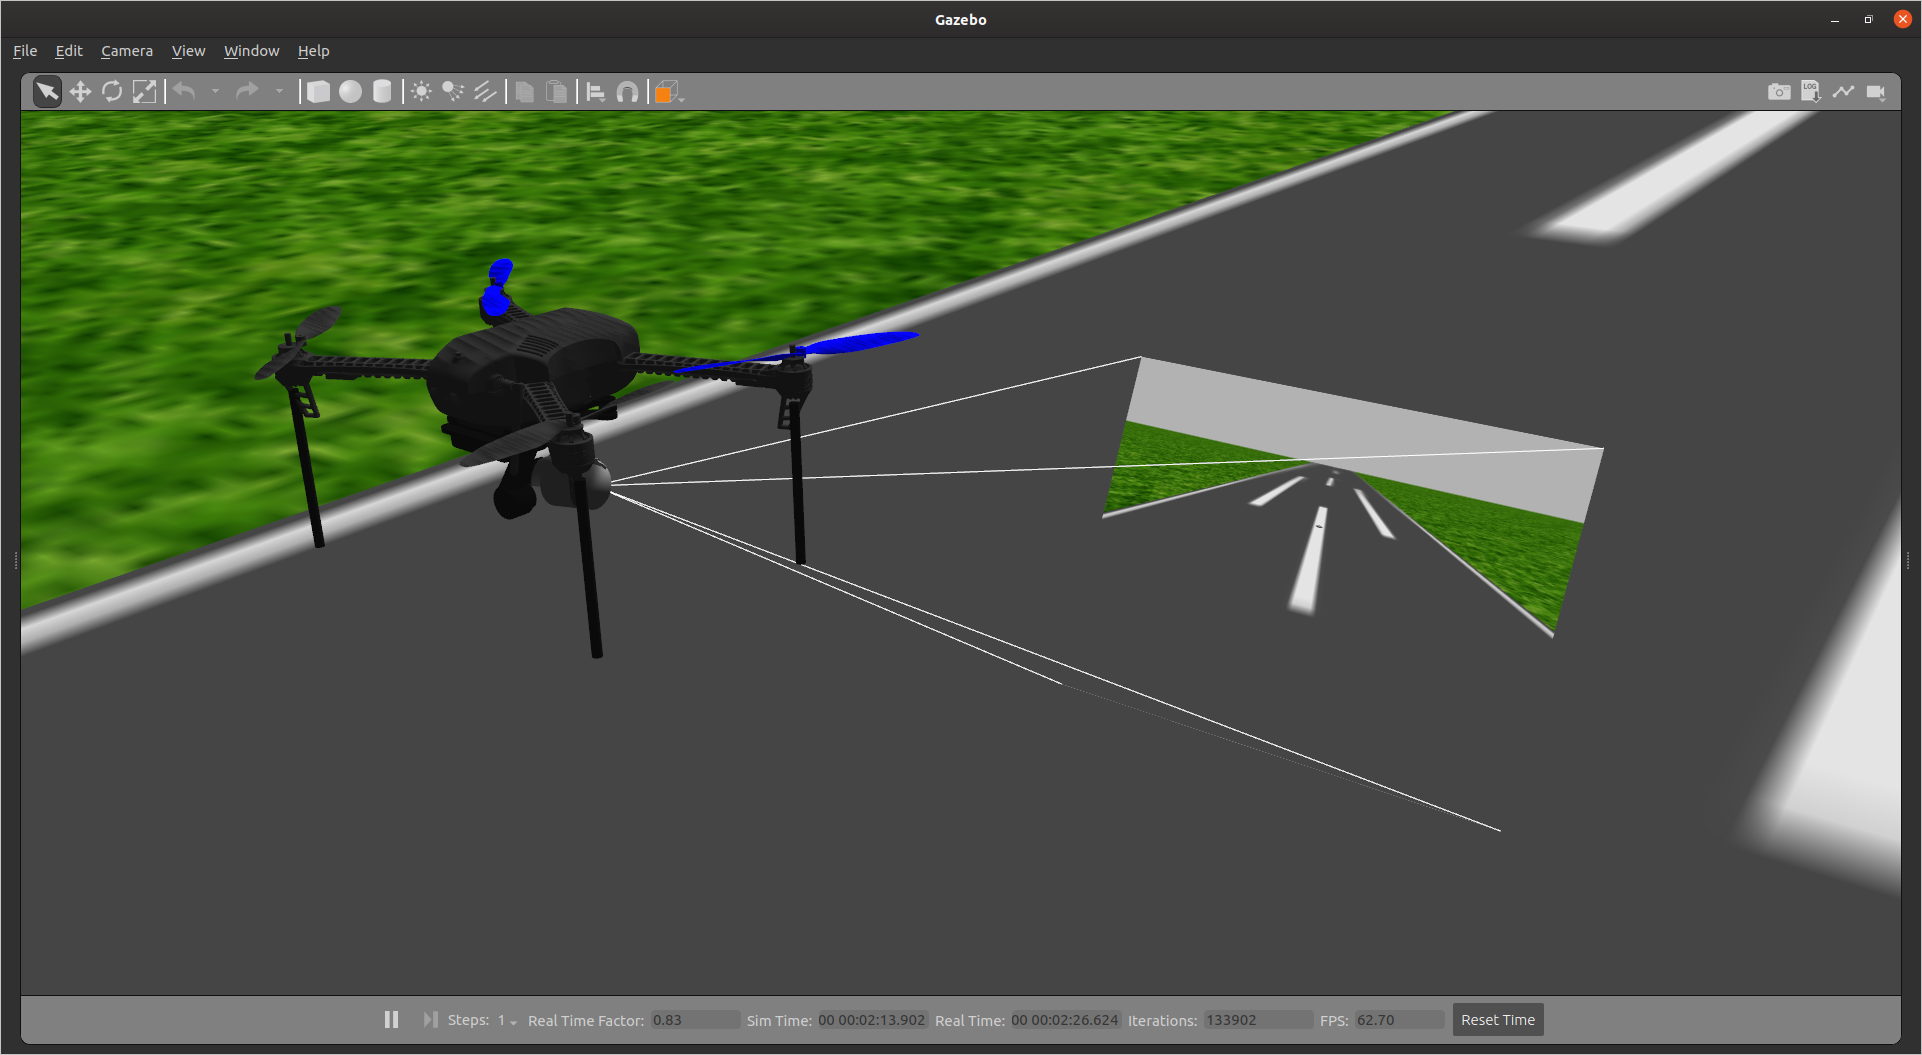
\includegraphics[width=0.6\textwidth]{images/gazebo_camera.png}
    \caption{The view of the drone's camera in Gazebo.}
    \label{fig:gazebo_camera}
\end{figure}

\subsubsection{\gls{GCS} Software}

The chosen \gls{GCS} software for this project, as mentioned in Section \ref{subsection:gcs}, is QGroundControl, which is depicted in Figure \ref{fig:qgroundcontrol}. There are several \gls{GCS} alternatives available open source. This particular one was chosen purely because of its ease of installation, but this choice is not important to the outcome of this project. It is only necessary to have some \gls{GCS} software, as it provides easy manual control of the drone in the absence of a conventional radio remote controller during simulation. This is important particularly in the early stages of testing, to perform ad hoc testing and to determine strategies for more formal, automated testing as will be described in Chapter \ref{chapter:simulation_results}.

\begin{figure}[ht]
    \centering
    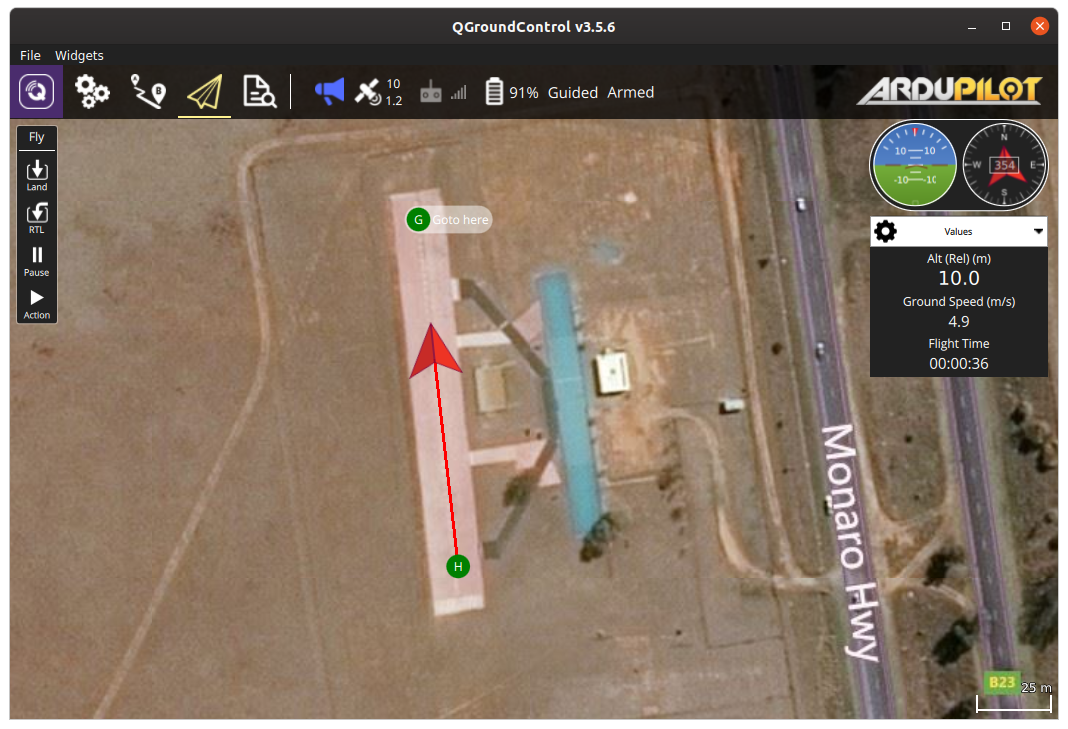
\includegraphics[width=0.6\textwidth]{images/qgroundcontrol.png}
    \caption{The QGroundControl software.}
    \label{fig:qgroundcontrol}
\end{figure}

% The landing area, shown in Figure \ref{fig:landing_pad} is comprised of two separate markers. The large circular WhyCon marker is used for long-range identification of the landing pad, as its simpler design and lack of inherent identifier make it easier to recognize from farther away. An April Tag marker is positioned in front of the landing pad, so that it will be visible throughout the drone's entire descent, albeit from a sharp angle of deflection. The April Tag's distinct identifier means that its unambiguous orientation can be determined reliably, even at sharp angles of deflection. This means that, once the large WhyCon marker has eclipsed the camera's field of view, the drone will still have reliable visual localization capabilities with which to estimate its position relative to the landing pad. More information on the theory behind these fiducial markers, as well as empirical comparisons of their performance are outlined in Section \ref{subsection:fiducial_markers}, and in the papers cited therein. Importantly, both of these fiducial systems have open-source ROS modules available, meaning that the development of a fiducial marker was not necessary for this project. The image from the simulated camera is provided as input to both fiducial systems, so that two different estimations of the landing pad's position are available. The dimensions and positions of the markers, and the distortion matrix of the camera are known to the landing system, so that the system can accurately estimate the landing pad's position. The drone targets the center of the WhyCon marker as its point of contact with the landing pad, and the gimbal controller generates a coordinate transform to align the drone with the center of the WhyCon marker using only the April Tag marker, when the WhyCon marker itself is not in view. 

% \begin{figure}
%     \centering
%     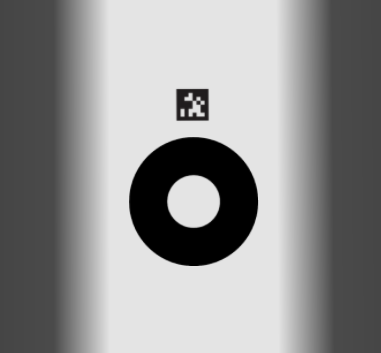
\includegraphics[width=0.6\textwidth]{images/landing_pad.png}
%     \caption{Landing pad design.}
%     \label{fig:landing_pad}
% \end{figure}

\section{Gimbal Controller}
\label{section:gimbal_controller}

\subsection{Overview}

In experiments using drones with a mounted camera, it is typical to see a camera with a fixed mounting angle. This provides simplicity in the estimation of the drone's pose relative to some fiducial marker, but limits the ability of the drone to detect the marker, as the drone itself must be facing the marker in order to detect it in the first place. A key aspect of this project is the development of a method for pose estimation of a drone relative to a fiducial marker using a gimbal-mounted camera for a wider range both of relative pose between the marker and the drone, and a wider range of acceptable behaviors for the drone during landing. This requires a slightly more involved system for coordinate transforms, as well a method for aiming the gimbal at the marker and tracking it over time.

\subsection{Data Flow}

\begin{figure}[ht]
    \centering
    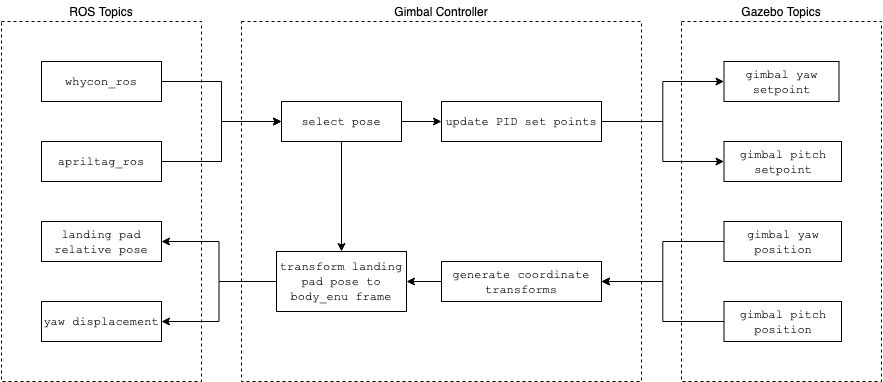
\includegraphics[width=\textwidth]{images/gimbal_controller_diagram.png}
    \caption{Gimbal controller data flow diagram.}
    \label{fig:gimbal_controller_diagram}
\end{figure}

The diagram in Figure \ref{fig:gimbal_controller_diagram} gives a high-level overview of the gimbal controller's functionality. The WhyCon and April Tag modules publish the pose of their possibly identified fiducial markers after analyzing the image from the simulated camera. If either module finds no marker in the image, then that module publishes no pose. If both markers are detected at the same time, only the April Tag marker is selected, and if only a WhyCon marker is detected, then it is used. The gimbal controller then updates the PID set points according to Equation \ref{equation:setpoints} and these are used by the PID controller instances in Gazebo. The gimbal controller subscribes to the true yaw and pitch positions of the gimbal, provided by Gazebo, which are not necessarily equal to the set points. These gimbal yaw and pitch positions provide the necessary information to generate the coordinate transform from the camera frame to the body ``ENU'' (East, North, Up) frame. The landing platform pose is then transformed to the body ENU frame and is published as its own topic. The ``yaw displacement,'' denoting the angle between the north axis of the drone and the north axis of the landing pad, is also published as a topic. 

The typical NWU (North, West, Up) coordinate system of Gazebo is visualized in Figure \ref{fig:nwu_coordinate_system}, with the red axis line pointing to the drone's ``north,'' the green axis line pointing to the drone's ``west,'' and the blue axis line pointing up. This is in contrast to the typical ROS \gls{ENU} coordinate system, in which the axis lines in Figure \ref{fig:nwu_coordinate_system} would be rotated by 90\degree clockwise in the ``up'' axis, so that the red axis points east, the green axis points north, and the blue axis points up. These lines represent the positive directions of their respective axes.

\begin{figure}[ht]
    \centering
    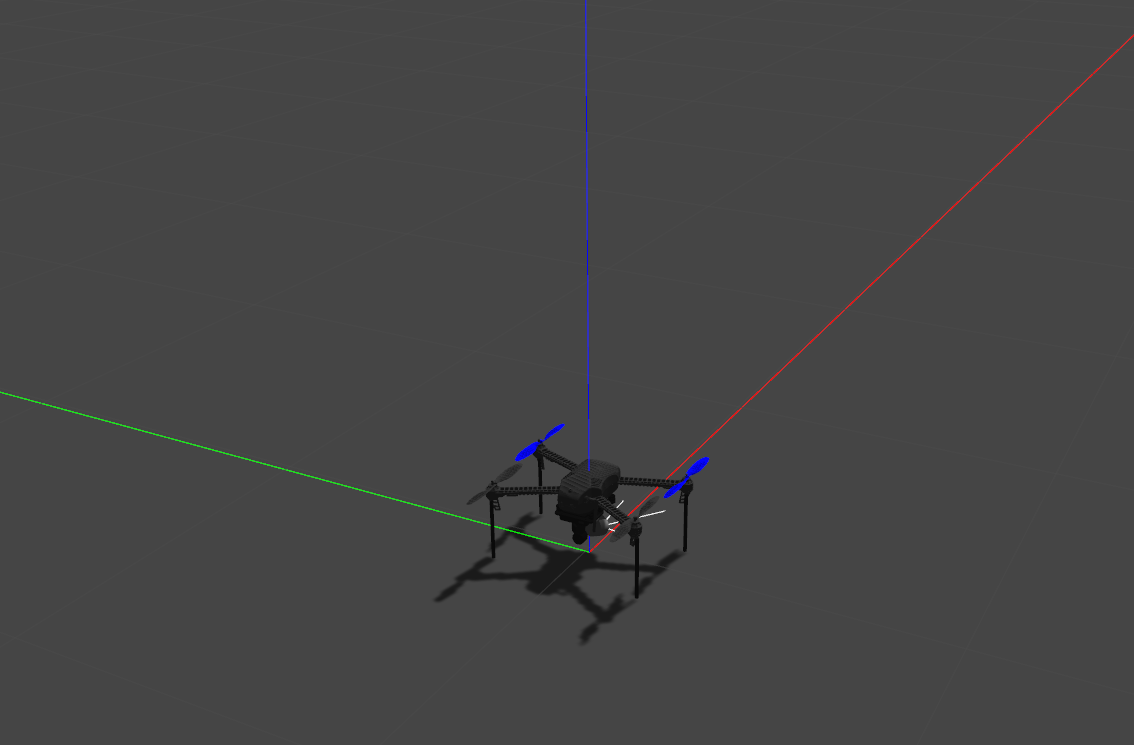
\includegraphics[width=0.6\textwidth]{images/nwu_coordinate_system.png}
    \caption{NWU (North, West, Up) Coordinate System within Gazebo.}
    \label{fig:nwu_coordinate_system}
\end{figure}

\subsection{PID Controllers for Gimbal Control}

\gls{PID} systems (outlined in Section \ref{section:pid_controllers}) provide a natural solution to the problem of aiming the gimbal, with the goal being to keep the marker in the center of the camera's field of view at all times. It would also be natural, therefore, to control the position of the camera based on the pixel positions of the detected fiducial markers. However, both the April Tag and WhyCon systems provide the positions of their markers in the form of a pose (\textit{not} pixel locations) - a specification of the linear translation and spacial orientation from the viewpoint to the marker. These poses are composed of a 3-dimensional vector providing the translation in (simulated) meters, and a quaternion providing the orientation. It is simple to control the position of the camera using the poses of the detected fiducial markers - instead of using pixel locations - in order to avoid additional edits to the already existing code, and also to avoid potentially required specificity to any hardware system (cameras may have different pixel ranges and therefore different centers).

\subsubsection{Gazebo Plugin Implementation for Gimbal Control}

A Gazebo plugin was added to the simulated drone's gimbal provide \gls{PID} control of the orientation of the gimbal and camera. The plugin is defined as a ROS module, is included in the model's definition \texttt{.sdf} file, and its library is loaded by Gazebo at runtime. This plugin subscribes to ``setpoint'' topics that are provided by the \texttt{gimbal\_controller} ROS module. As the gimbal has 2 degrees of freedom (yaw and pitch), 2 corresponding \gls{PID} controllers set the orientation of their respective gimbal axes. The gimbal has artificial limits of $\theta_{yaw} \in \left[ -\frac{\pi}{2}, \frac{\pi}{2} \right]$ and $\theta_{pitch} \in [0, \pi]$ for simplicity. $\theta_{yaw} = 0$ describes a situation where the camera is pointing directly forward (with respect to the drone's local coordinate frame), and $\theta_{yaw}$ increases as the camera rotates clockwise. $\theta_{pitch} = 0$ describes a situation where the camera is pointing forward, directly level to the drone. $\theta_{pitch}$ increases as the camera rotates towards vertical-down. The 2 \gls{PID} controllers are able to control the position of the camera only in these ranges, which helps the system to avoid unnecessary rotations during simulation and also mimics the natural limits of physical systems. The gains of these systems were determined experimentally and will be described in Section \ref{subsection:pid_tuning}. The plugin also publishes the true angles of the gimbal in each dimension as ROS topics for the subsequent calculation of coordinate transforms, explained in Section \ref{subsection:coordinate_system_transforms}.

\subsection{Aiming the Camera}
\label{subsection:aiming_the_camera}

The gimbal controller has callback functions for both WhyCon and April Tag detections, where it updates the set points (target states) of both \gls{PID} controllers. Let $SP_x$ be the set point of the gimbal's yaw axis, and let $SP_y$ be the set point of the gimbal's pitch axis. The yaw and pitch axes of the gimbal can be visualized in Figure \ref{fig:gazebo_camera}, where the yaw of the gimbal is in line with the yaw of the drone ($\theta_{yaw}=0$), and the pitch of the gimbal is slightly less than that of the drone ($\theta_{pitch} > 0$). Then, upon detection of a fiducial marker, the set points are updated as in equation \ref{equation:setpoints}:

\begin{equation}
    \begin{array}{l}
        SP_x = SP_x - k \frac{x}{z} \\
        SP_y = SP_y + k \frac{y}{z}
    \end{array}
    \label{equation:setpoints}
\end{equation}

where $k$ is an experimentally determined scalar, and $x,y,z$ are the linear components of the marker's pose in the west, down, and north axes of the camera respectively. The callback functions \textit{increment} the set points instead of calculating them directly. The difference in the sign of the increment occurs because of the specific nature of Gazebo's axis conventions. This particular aspect would require special attention and verification when transitioning to a real world environment. The increment is scaled inversely to $z$ in order to ensure that the system works over a range of distances. 

\subsection{Landing Pad Design and Prioritization of Fiducial Marker Detections}
\label{subsection:landing_pad_design}

\begin{figure}[ht]
    \centering
    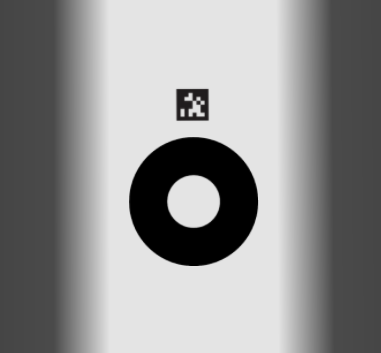
\includegraphics[width=0.6\textwidth]{images/landing_pad.png}
    \caption{Landing pad design.}
    \label{fig:landing_pad}
\end{figure}

As shown in Figure \ref{fig:landing_pad}, the landing pad is made up of two markers. The system recognizes the larger (1 meter in diameter), more easily identifiable WhyCon marker before it recognizes the April Tag marker (with side length 0.3125 meters). However, since the April Tag marker is used for final descent at close range, the gimbal controller prioritizes the April Tag marker over the WhyCon marker. So in the case that both markers are visible, the gimbal controller aims the camera at the April Tag marker. If the April Tag marker becomes obstructed, the gimbal controller then aims the camera at the WhyCon marker again. This prioritization is illustrated in Figure \ref{subfig:whycon_detection_only} through \ref{subfig:centered_april_tag_detection}. In the detection windows, detected WhyCon markers are highlighted, and detected April Tag markers have their IDs printed above the marker itself. The fact that the April Tag marker is flat on the landing pad's plane does mean that, at a low altitude, it will be somewhat difficult to recognize the April Tag's pose. However, this is a challenge to overcome anyway, as it keeps the landing pad simple and completely flat (and therefore free of obstructions). The center of the April Tag marker is positioned 0.75 meters north of the center of the WhyCon marker. This allows for the marker to be adequately close to the drone during final descent that it can always be easily recognized. However it also means that the April Tag marker is adequately displaced from the camera to always be in the camera's field of view. This distance is likely to be adjusted in real world experiments. The original design for the landing platform included only a single WhyCode marker, but this was abandoned for reasons that will be discussed in Section \ref{subsection:whycode_trials}.

% \begin{figure}
%     \centering
%     \subfloat[WhyCon detection only.\label{subfloat:whycon_only}]{{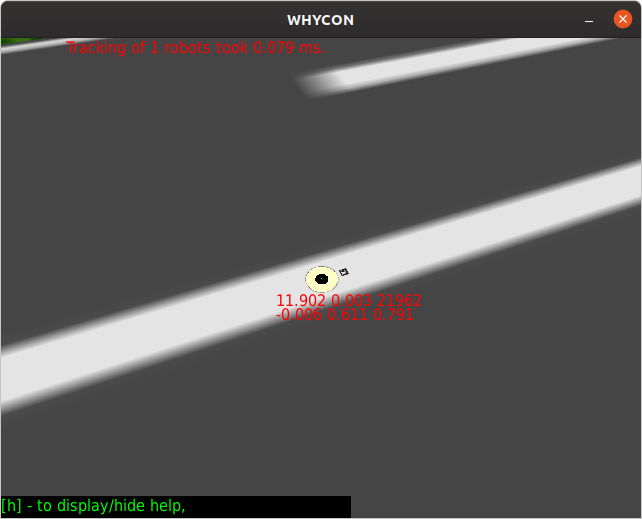
\includegraphics[width=0.45\textwidth]{images/whycon_detection_only.png} }}
%     \hfill
%     \subfloat[No April Tag detection.\label{subfloat:no_apriltag}]{{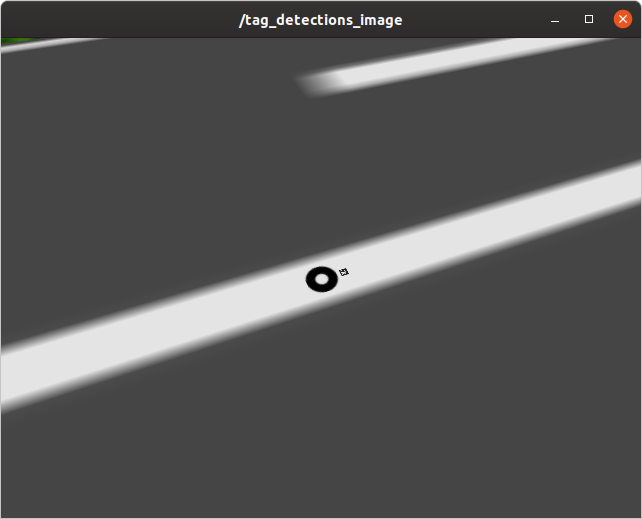
\includegraphics[width=0.45\textwidth]{images/no_apriltag.png} }}\\
%     \subfloat[Off-center WhyCon detection.\label{subfloat:off_center_whycon}]{{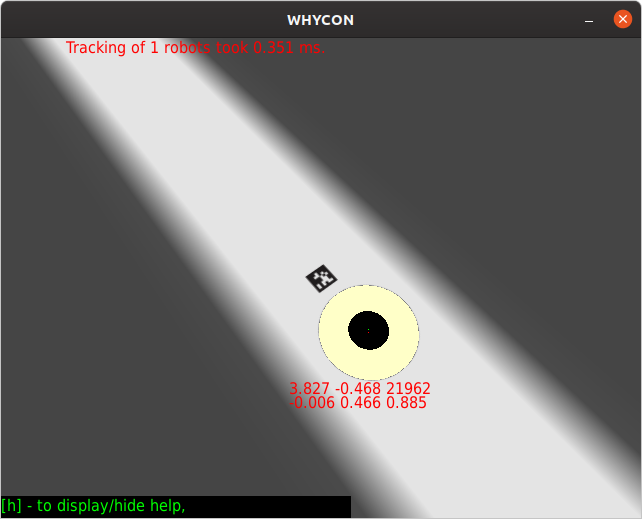
\includegraphics[width=0.45\textwidth]{images/whycon_off_center.png} }}
%     \hfill
%     \subfloat[Centered April Tag detection.\label{subfloat:apriltag_detection}]{{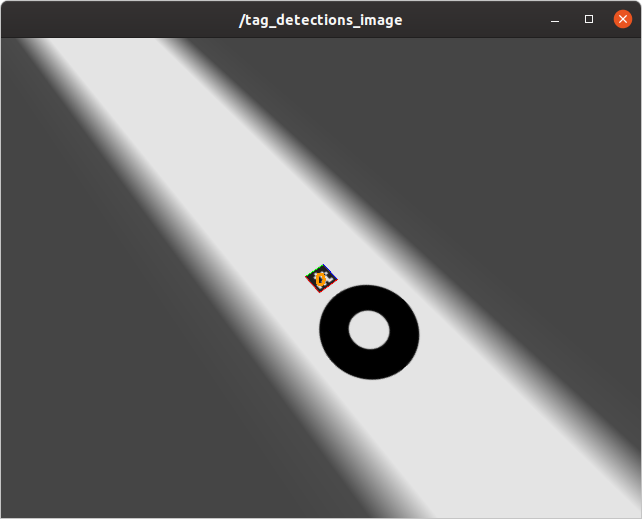
\includegraphics[width=0.45\textwidth]{images/apriltag_detection.png} }}
% \end{figure}

% [height=6.5cm]

\begin{figure}
     \centering
     \begin{subfigure}[b]{0.49\textwidth}
         \centering
         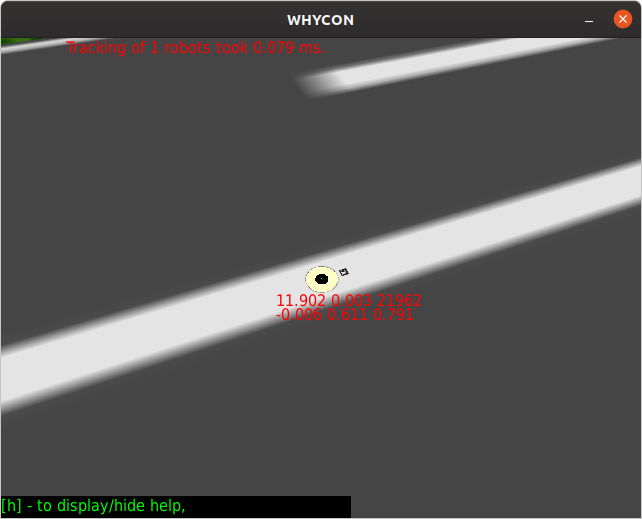
\includegraphics[width=\textwidth]{images/whycon_detection_only.png}
         \caption{WhyCon detection only.}
         \label{subfig:whycon_detection_only}
     \end{subfigure}
     \hfill
     \begin{subfigure}[b]{0.49\textwidth}
         \centering
         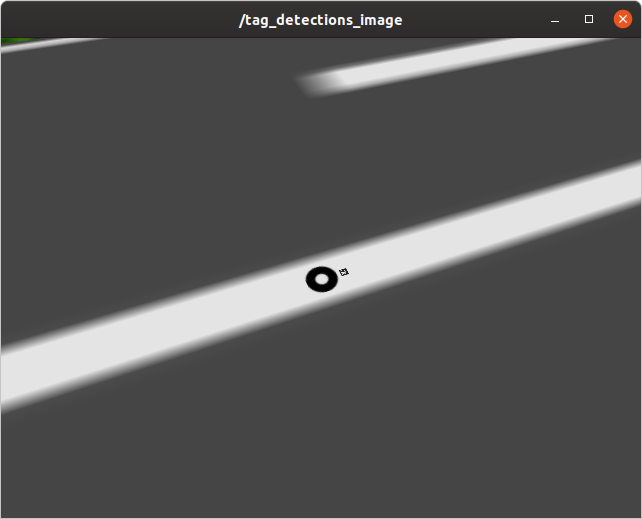
\includegraphics[width=\textwidth]{images/no_apriltag.png}
         \caption{No April Tag detection.}
         \label{subfig:no_apriltag_detection}
     \end{subfigure}
     \begin{subfigure}[b]{0.49\textwidth}
         \centering
         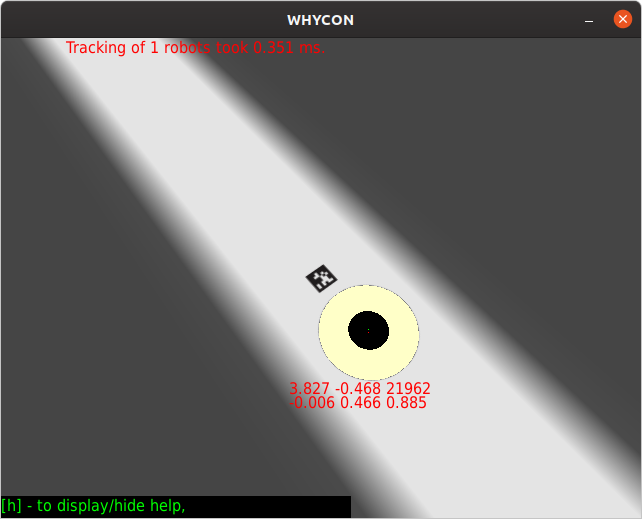
\includegraphics[width=\textwidth]{images/whycon_off_center.png}
         \caption{Off-center WhyCon detection.}
         \label{subfig:off_center_whycon_detection}
     \end{subfigure}
     \hfill
     \begin{subfigure}[b]{0.49\textwidth}
         \centering
         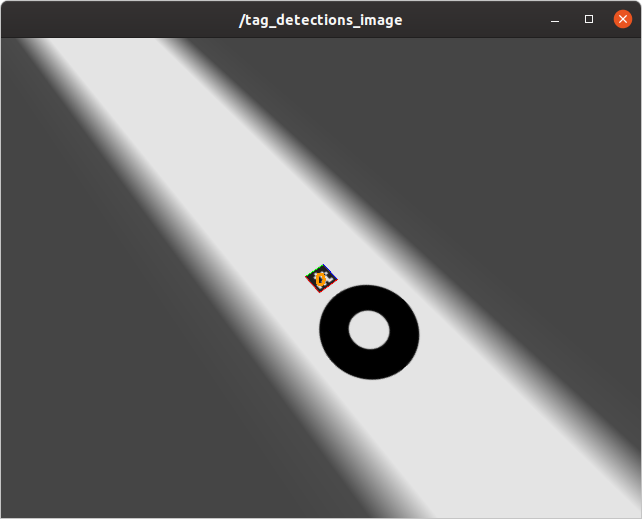
\includegraphics[width=\textwidth]{images/apriltag_detection.png}
         \caption{Centered April Tag with ID ``0'' overlayed.}
         \label{subfig:centered_april_tag_detection}
     \end{subfigure}
        \caption{Prioritization of fiducial marker detections.}
        \label{fig:detections}
\end{figure}

A Gazebo model of the landing pad allows for control of the landing pad's velocity. It is essentially the same as the original landing pad, with the difference that the fiducial marker textures are added to a model with two collision planes, to simulate an entity separate from the ground. The friction is set quite high on the top collision plane ($\texttt{mu} = \texttt{mu2} = 100000$), in order to avoid artificial slipping of the drone on the landing pad, which would not happen on a properly designed physical landing pad. The friction on the lower collision plane is set to 0 in order to avoid unintended bouncing and extraneous drag effects which result from interaction with the ground collision plane. A separate Gazebo plugin controls the linear and angular velocity of the landing pad via ROS topics. It is necessary to continually set the velocity of the landing pad even in stationary landing situations, as the forces applied by the drone upon contact can cause the landing pad to sink into the ground, even with well-defined collision planes. The drone then detects this movement and attempts to correct, resulting in unintended behavior. Setting the velocity of the landing pad avoids this issue. In \texttt{sandbox.world}, the parameter \texttt{contact\_surface\_layer} was increased to 0.01 in order to avoid further bouncing between the drone and the landing pad itself. The landing platform model is shown in Figure \ref{fig:landing_pad_model}. The size of the WhyCon marker (where the drone is supposed to land) is 1 meter in diameter, while the drone legs are roughly positioned at the corners of a rectangles with side lengths 0.44 meters and 0.26 meters. This allows the drone to fit entirely on the WhyCon marker with space to spare, while still keeping the landing platform small enough to be manageable in the real world, in scenarios where it can be mounted to the top of a car or bus, or simply positioned on the ground.

\begin{figure}
    \centering
    
\includegraphics[width=0.5\textwidth]{images/landing_pad_model.png}
    \caption{The separate landing pad model.}
    \label{fig:landing_pad_model}
\end{figure}

The landing pad velocity controller plugin subscribes to a topic \texttt{/landing\_pad/cmd\_vel} of type \texttt{geometry\_msgs/Twist}, the components of which specify the components of the landing platform velocity in each of the 3 dimensions. A callback function within the plugin sets the values in the Gazebo engine, and also sets the value of the landing pad's angular velocity to 0 in all directions. This conforms to the assumption that the velocity of the landing pad will be predictable and cooperative from the point of view of the drone. The velocity of the landing pad is set manually during testing, from the terminal using the \texttt{rostopic pub} command. This is published at a high frequency in order to negate extraneous physics effects.

\subsection{Coordinate System Transforms}
\label{subsection:coordinate_system_transforms}

The second function of the gimbal controller is to generate coordinate system transforms based on the position of the gimbal. This is necessary because the camera is almost never directly in line with the drone's axis system, as shown in Figure \ref{fig:camera_offset}. The blue propellers indicate the front of the drone, and the camera is offset counter-clockwise and down so that it may point at the detected fiducial markers.

\begin{figure}
    \centering
    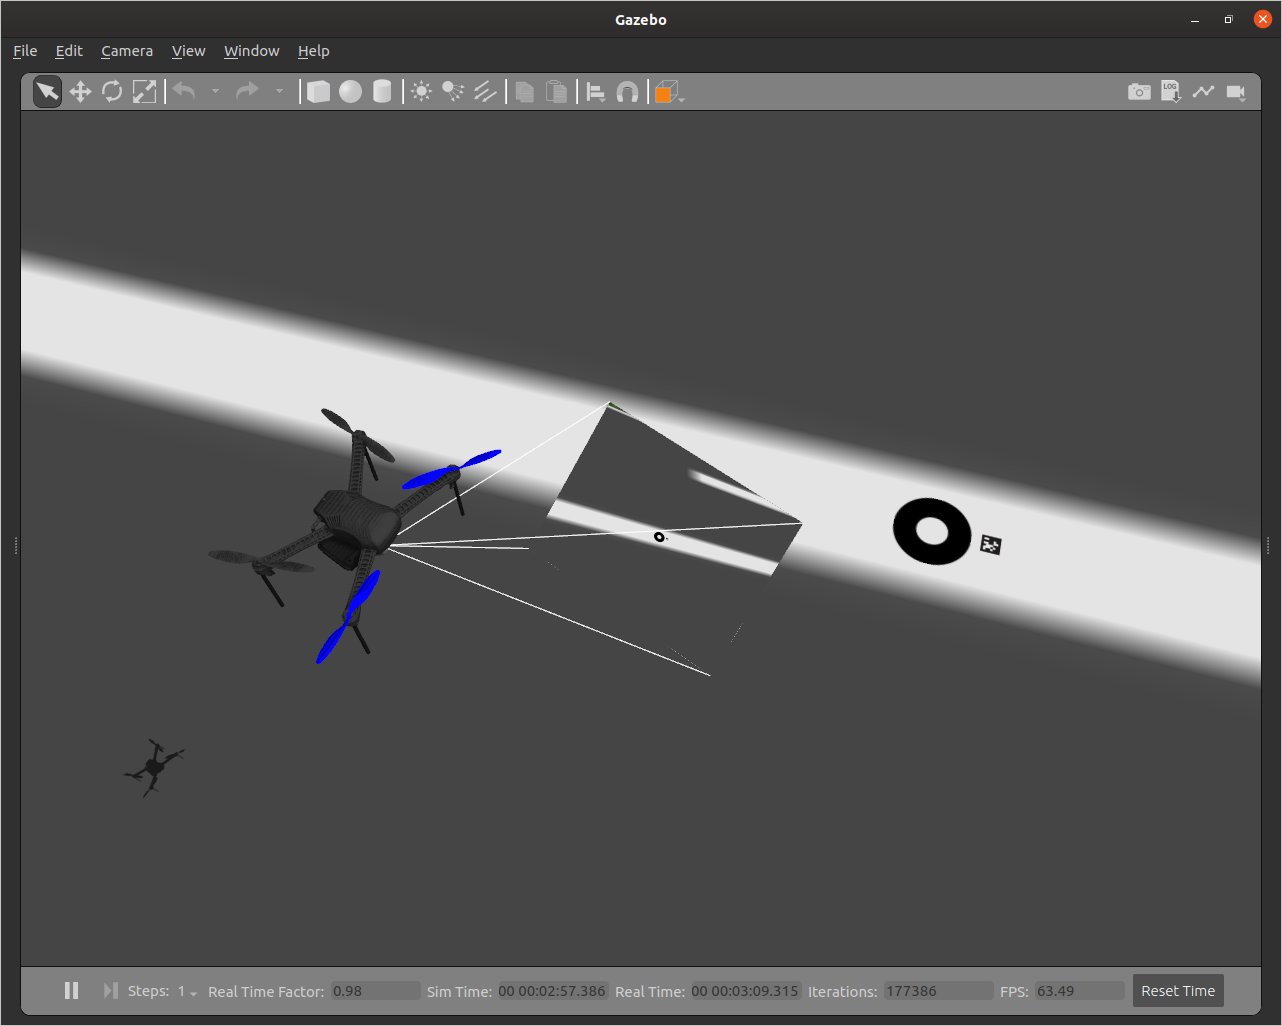
\includegraphics[width=0.8\textwidth]{images/gimbal_controller.png}
    \caption{Illustration of the drone after detecting the landing pad.}
    \label{fig:camera_offset}
\end{figure}

The role of the transforms in this scenario is to take into account the rotational displacement of the camera with respect to the drone's intrinsic, local axes, so that the pose of the landing pad can be calculated in terms of the drone itself. As a simple example to illustrate this point: if the camera is rotated to $\theta_{yaw}=-\frac{pi}{2}$ and $\theta_{pitch}=\frac{pi}{4}$, and a marker is detected 10 meters forward (in the camera's coordinate system), the gimbal controller generates a transform that will place the marker 10 meters to the left of the drone. Since the gimbal has only 2 degrees of freedom, the gimbal controller can generate the relevant transform using only the supplied pitch and roll topics from the gimbal controller plugin. This structure corresponds to a real world scenario wherein the gimbal has a mounted \gls{IMU} from which the corresponding values can be extracted.

Although the yaw position of the camera is a truly necessary component of determining the relative pose with a rotating gimbal, the pitch is not. A second method of pose estimation in this scenario is therefore to ``straighten'' the detected pose, so that the orientation is in the reference frame of the fiducial marker's normal vector. The result is that the marker's rotation is no longer needed in subsequent calculations, and the translational elements of the pose correspond to the distances in the 3 dimensions of a coordinate system centered on the marker. This can be accomplished by simply creating a transform whose translational element $t = <0, 0, 0>$ (no translation), and whose rotational element is the inverse of the marker's rotation in the original pose frame. After this transform is generated, a second transform corrects for the yaw displacement of the camera. In the case of a WhyCon marker which has no intrinsic origin in terms of yaw, a second transform corrects for the yaw displacement of the camera by adding a rotation equal to the inverse of the camera's yaw. In the case of a WhyCode or April Tag marker which do intrinsically have unambiguous yaw orientations in their pose, the yaw used to correct the pose is equal to the difference between the gimbal's yaw displacement and the marker's yaw displacement. The inverse of this value is the rotational component of the second transform. If $\theta_1$ represents the yaw of the camera, $\theta_2$ represents the yaw of the marker, and $\theta_c$ represents the yaw used to correct the pose, then $\theta_c$ can be simply calculated as follows in equation \ref{equation:yaw_correction}. In the case of a WhyCon marker, $\theta_2$ is just 0.

\begin{figure}[ht]
    \centering
    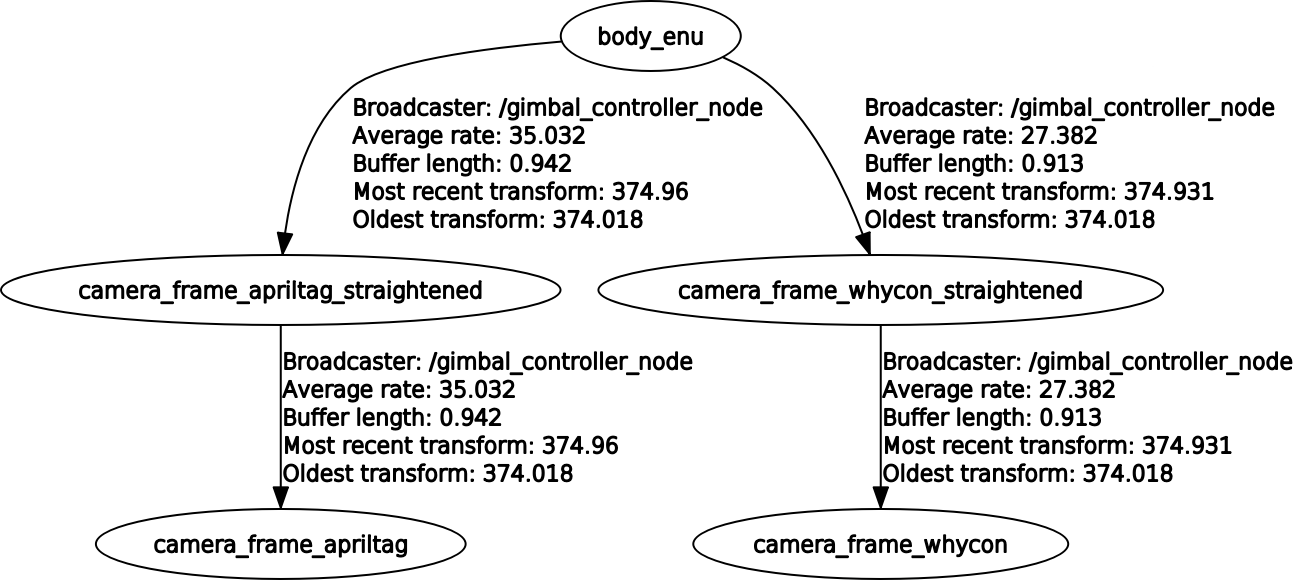
\includegraphics[width=0.7\textwidth]{images/transform_tree.png}
    \caption{Transforms used for calculating the drone's pose relative to the landing pad.}
    \label{fig:transform_tree}
\end{figure}

Figure \ref{fig:transform_tree} shows the transforms involved in calculating the drone's position relative to the April Tag or WhyCon markers. Each node contains the name of the transform frame. The function of each frame is as follows:

\begin{enumerate}
    \item \texttt{camera\_frame\_apriltag}: the transform representing the pose of the April Tag marker within the camera's field of view. This is taken from the April Tag ROS module which is analyzing the camera's published image.
    \item \texttt{camera\_frame\_apriltag\_straightened}: the transform representing the April Tag's pose when transformed to have a rotation quaternion of $\left( x, y, z, w \right) = \left( 0, 0, 0, 1 \right)$. This essentially gives the pose of the camera with respect to the marker. If the rotation of the April Tag marker in the camera's field of view is $r_a$, then this transformation composes a rotation of $r_a^{-1}$. In this case, since the April Tag's pose has unambiguous yaw, the yaw is included in this calculation.
    \item \texttt{camera\_frame\_whycon}: the transform representing the pose of the WhyCon marker within the camera's field of view. Since the WhyCon marker does not have an unambiguous yaw position, this aspect of the pose is ignored. This is taken from the WhyCon ROS module which is analyzing the camera's published image.
    \item \texttt{camera\_frame\_whycon\_straightened}: the transform representing the pose of the camera with respect to the WhyCon marker. This is calculated similarly to the straightened April Tag transform, but without considering the yaw of the marker. 
    \item \texttt{body\_enu}: the pose of the drone itself with respect to either the WhyCon or April Tag marker. This is calculated by composing the yaw component of the gimbal's rotation onto the previously straightened transforms. The relative displacement from the marker to the drone can be used in further calculations after it is transformed in this way. It is put in the \gls{ENU} coordinate frame in order to conform to the MAVROS standard.
\end{enumerate}

The transform library TF2 (used here) is the standard ROS transform library and provides an efficient means of keeping track of all published transforms 

\begin{equation}
    \theta_c = -\left( \theta_1 - \theta_2 \right)
    \label{equation:yaw_correction}
\end{equation}

When the drone is far from the landing pad and only the WhyCon marker can be identified, the gimbal controller cannot determine any information about the yaw orientation of the landing platform. This is because the WhyCon marker has rotational symmetry. Initially, the landing platform was made up of a WhyCode marker which can allow for determination of the marker's yaw orientation. However, this led to complications and was eventually abandoned for this project, as will be explained in Section \ref{subsection:whycode_trials}. The current landing platform design, using a WhyCon marker for recognition of the landing pad from a far distance, and an April Tag marker for close-range descent and accurate pose estimation, is sufficient for this project.

\section{Landing Controller}
\label{subsection:landing_controller}

\subsection{Overview}
The landing controller is a \gls{ROS} module which controls the drone's approach and descent towards the landing platform. It subscribes to data topics published by the gimbal controller, such as the relative displacement of the landing pad with respect to the drone. Then the landing controller determines the commands to send to ArduPilot in order to direct the drone towards the landing pad. It communicates with ArduPilot via a separate \gls{ROS} module called \texttt{MAVROS}, the sole purpose of which is to act as a connector between \gls{ROS} modules and any vehicle using the MAVlink communication protocol. The \texttt{MAVROS} module opens the relevant \gls{UDP} or \gls{TCP} connections with instances of MAVlink-enabled software and enables transmission of data to and from these connections via \gls{ROS} topics. These connections allow the landing controller to send control commands to the drone in the language of the flight controller, without changing the software on the flight controller.

\subsection{Data Flow}

\begin{figure}[ht]
    \centering
    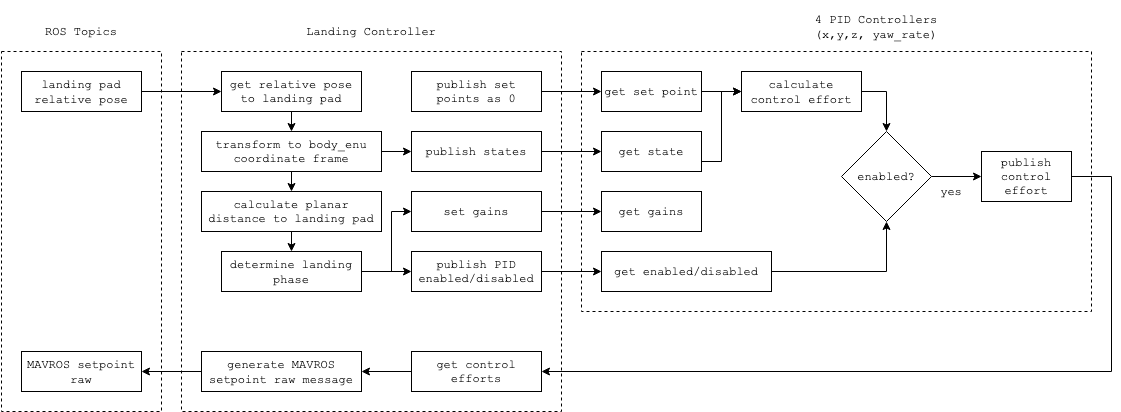
\includegraphics[width=\textwidth]{images/landing_controller.png}
    \caption{Data flow for the landing controller.}
    \label{fig:landing_controller_data_flow}
\end{figure}

The data flow for the landing controller is shown in Figure \ref{fig:landing_controller_data_flow}. The landing controller subscribes to a ROS topic containing the relative pose from the drone to the landing pad. It then transforms this pose from the camera's coordinate frame to the drone's local coordinate frame, using transforms that are also published by the gimbal controller. The landing controller publishes the states for each linear component of the displacement to each of the PID controllers. It also continually publishes the set points for the PID controllers - each with a value of 0. The planar distance to the landing pad is calculated from the relative pose, and this subsequently determines the landing phase and therefore the gains of the PID controllers and whether the PID controllers should be enabled or disabled. The PID controllers subscribe to this data, calculate the corresponding control efforts and publish the control efforts if they are enabled. Finally, the landing controller subscribes to the control effort topics, generates a message to be consumed by MAVROS, and publishes that message.

\subsection{Velocity PID Controllers}

\gls{PID} controller instances control the velocity of the drone in 4 axes that are local to the drone: east, north, up, and yaw (positive yaw is clockwise). The state values for these controllers are the component of the drone's displacement from the landing pad in the relevant axis. Since the goal of the landing controller is to direct the drone towards the landing pad - in other words, to decrease the magnitude of the displacement - the landing controller continually publishes 0 as the set point to each of these controllers when they are active. A control policy both enables/disables these controllers and changes the gains of these controllers based on the phase of the landing process. The \gls{PID} controllers publish their ``control effort'' topics after receiving data on their state and set point topics. These control effort topics are of course determined according to their gains. The landing controller subscribes to the control effort topics and translates these into a control message which is passed to ArduPilot via MAVROS.

\subsection{MAVROS Interface}

MAVROS handles communication between ROS and ArduPilot by translating ROS topics into MAVLink messages. For controlling position, velocity, and acceleration set points, the topic of interest is \texttt{/mavros/setpoint\_raw/local}. This topic allows ROS to forward the target velocities that are calculated by the PID controllers to the drone itself. This does mean that there are two sets of PID controllers - one set which calculates the target velocities, and one set that realizes these target velocities by setting the lower-level \gls{PWM} throttle signals on the drone itself, while interfacing with the \gls{IMU} to control otherwise unspecified targets such as attitude, acceleration, etc. This abstraction from the low-level commands is what allows the landing controller to be portable to different drone models and frames. The drone's intrinsic PID controllers which maintain the stable, controllable flight of the drone are tuned for their specific tasks, and the higher level PID systems are tuned for the specific task of realizing an efficient and safe trajectory towards the landing platform.

Listing \ref{lst:set_velocity_target_neu} shows the method for sending the control message to the drone. The target velocity and yaw rate represent the control effort variables calculated by the PID controllers. The \texttt{/mavros/setpoint\_raw/local} topic receives a message of type \texttt{PositionTarget}, for which a buffer has been declared. The message is stamped with the current time and tagged with the frame identifier of ``world.'' Multiple coordinate frames are available for the interpretation of the set points, but the only relevant one for this project is the coordinate frame that is local to the drone: \texttt{FRAME\_BODY\_NED} with code 8. A type mask tells the drone which parts of the message are relevant - in this case, only the linear velocities $x,y,z$ and yaw rate are published, so a value of 1991 is used. The message is then published to the topic.
\begin{lstlisting}[style=C++,caption={The simple function that allows the landing controller to control the drone's target velocities.},captionpos=b,label={lst:set_velocity_target_neu}]
void set_velocity_target_enu( geometry_msgs::Vector3 _target_velocity,
                              double _target_yaw_rate )
{
	mavros_msgs::PositionTarget buffer;

	buffer.header.stamp = ros::Time::now();
	buffer.header.frame_id = "world";
	buffer.coordinate_frame = 8; // FRAME_BODY_NED
	buffer.type_mask = 1991; // only use velocity x, y, z, yaw_rate

	buffer.velocity.x = _target_velocity.x;
	buffer.velocity.y = _target_velocity.y;
	buffer.velocity.z = _target_velocity.z;

	buffer.yaw_rate = _target_yaw_rate;

	setpoint_raw_local_publisher.publish(buffer);
}
\end{lstlisting}

There is some tedium in this setup which must be considered. First, the standard coordinate system within Gazebo is \gls{NWU}, while the standard coordinate system within MAVlink is \gls{NED}. While these are both right-handed coordinate systems and therefore a ``typical'' and simple transformation (a rotation by $\pi$ radians about the N axis) can be used, it is easier to manually change the signs of the corresponding components of the target velocity vector. Further, although MAVLink typically uses the \gls{NWU} coordinate system, MAVROS itself takes the target velocity vector in the \gls{ENU} coordinate system, which is not necessarily obvious from the documentation. However, when these aspects are accounted for, the software works as intended.

% \subsection{\color{red}Sensor Fusion and Filtering}

% {\color{red}Here I will discuss the method for sensor fusion likely using the \texttt{robot\_localization} or \texttt{robot\_pose\_ekf} ROS packages. I have attempted to use these packages already but failed to get decent results. After some time the ``filtered'' pose estimates start having a lot of spikes and become incredibly inaccurate. The goal is to be able to fuse the WhyCon, April Tag, and IMU sensor readings into a single landing pad estimate.}

\subsection{Control Policy}
\label{subsection:control_policy}

The landing controller enables/disables the PID controllers and changes their gains depending on conditions during the landing process. Initially the drone's velocity controllers have high P-gains and low D-gains. This allows the drone to approach the landing pad quickly from far distances. As the drone gets closer to the landing pad, the I and D gains become more important and are set to experimentally-determined values (presented in Section \ref{subsection:pid_tuning}) to avoid the quintessential PID overshoot and instead conserve battery and time. The standard ROS PID module has been slightly modified to allow the gains to be reconfigured quickly using a single topic, rather than the existing method of using \texttt{rqt\_reconfigure} which requires a separate module and which seems to react slowly to the reconfiguration.\footnote{The original PID module code can be found at \url{https://bitbucket.org/AndyZe/pid/src/master/} and the slightly edited version can be found at \url{https://github.com/uzgit/pid}.}

Although a drone can move in any direction, it is necessary to control the yaw of the drone during descent, as the legs of the drone can obstruct the tracked fiducial marker. Although WhyCon markers tend to be robust to minor obstructions, the more intricate April Tag markers are not. The Iris, for example, has a black airframe which can merge with the black boundary and tiles of April Tag markers in the field of view of the camera, forming a contiguous black region which does not conform to the required structure of April Tag markers and prevents April Tag identification. Figure \ref{fig:obstruction} illustrates this point. In Figure \ref{subfig:apriltag_not_obtructed}, the April Tag marker is clearly identified (hence the ID is printed on the screen) even at a somewhat high angle of deflection, but in Figure \ref{subfig:apriltag_obtructed}, the slight intersection of the drone's leg with the April Tag marker prevents identification. In this case, yaw correction  ensures that the drone is aligned to the landing platform in such a way that the April Tag marker is unobstructed by the drone itself throughout the descent. However, yaw correction is only allowed once the April Tag marker has been identified, since the April Tag marker is the only marker on the landing pad which provides a yaw orientation. In contrast to April Tag's obvious sensitivity, Figure \ref{fig:whycon_robust} shows the robustness of WhyCon identification. The shadow of the drone forms a contiguous black region extending the WhyCon marker's black region. (White and black are inverted in the picture in order to make the detection more clear.) However, the WhyCon system still correctly identifies the marker and places its center in the correct location, as shown by the very faint green and red dots.

\begin{figure}[ht]
    \centering
    \begin{subfigure}[b]{0.49\textwidth}
        \centering
        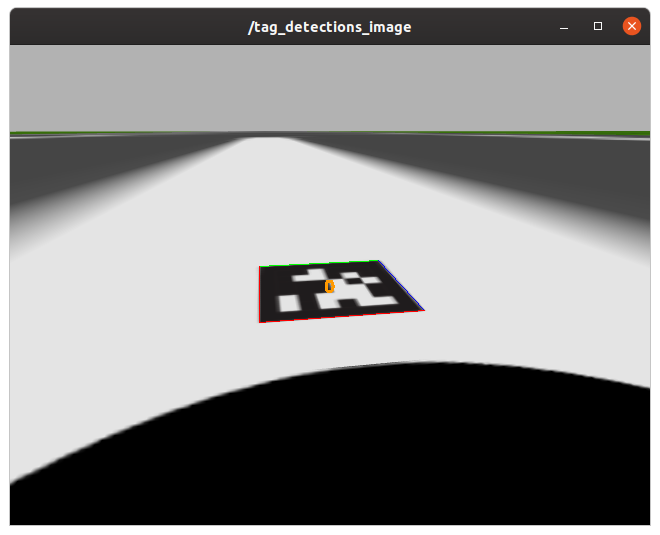
\includegraphics[width=\textwidth]{images/apriltag_not_obstructed.png}
        \caption{April Tag not obstructed, and therefore successfully identified.}
        \label{subfig:apriltag_not_obtructed}
    \end{subfigure}
    \begin{subfigure}[b]{0.49\textwidth}
        \centering
        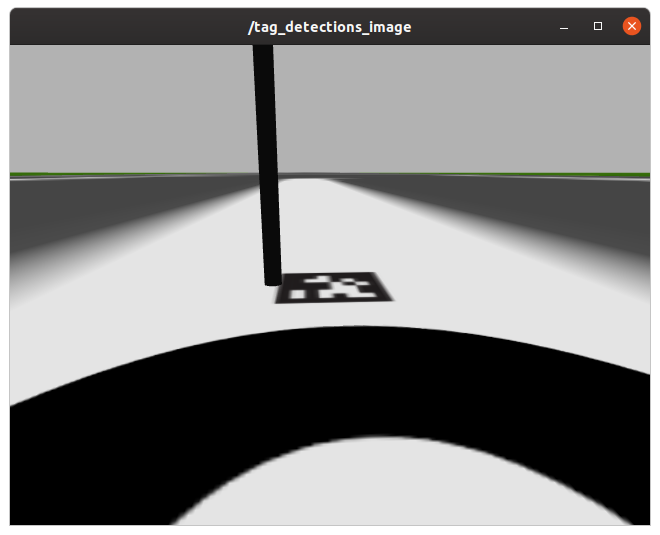
\includegraphics[width=\textwidth]{images/apriltag_obstructed.png}
        \caption{April Tag slightly obstructed, and therefore not identified at all.}
        \label{subfig:apriltag_obtructed}
    \end{subfigure}
    \caption{Even slight obstructions can prevent identification of April Tag markers.}
    \label{fig:obstruction}
\end{figure}

\begin{figure}[ht]
    \centering
    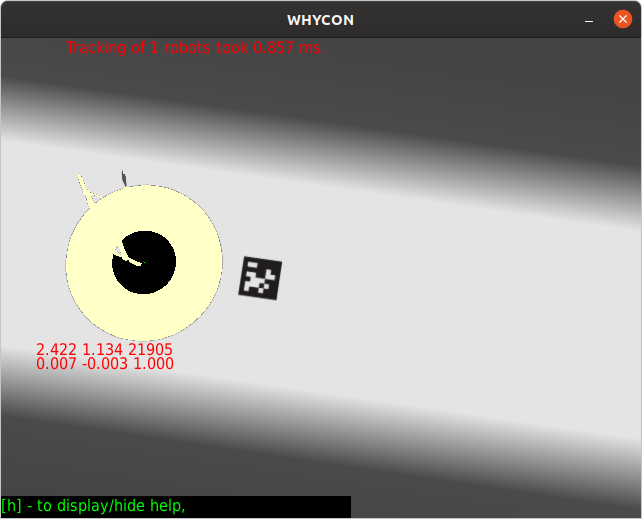
\includegraphics[width=0.5\textwidth]{images/whycon_robust.png}
    \caption{WhyCon identification is robust even to significant obstructions.}
    \label{fig:whycon_robust}
\end{figure}

Finally, descent is allowed or disallowed based on a dynamic threshold $\delta$ on the planar distance $d_p$ to the landing pad. This threshold follows an exponential function as outlined in Equation \ref{equation:plane_distance_threshold}:

\begin{equation}
    \delta = k_1e^{k_2 z}
    \label{equation:plane_distance_threshold}
\end{equation}
where
\begin{itemize}
    \item $\delta$ is the planar distance threshold, below which the drone is allowed to descend,
    \item $k_1$ and $k_2$ are constants determined through exponential fitting of a curve to experimentally-determined constraints, and
    \item $z$ is the vertical distance from the drone to the landing pad, or equivalently the altitude of the drone above the landing pad.
\end{itemize}

The drone is allowed to descend if $d_p = \sqrt{x^2 + y^2} < \delta$, where $x$ and $y$ are the distances from the drone to the landing pad in the drone's East and North axes respectively. This means that, the higher the drone is above the landing pad, the farther away it is allowed to descend. Conversely, the lower the altitude of the drone, the closer the drone must be to landing pad in order to descend - ensuring that the drone does not descend to the ground in any place except for the landing pad. This is visualized in Figure \ref{fig:descent_region}, where the descent region is the interior of the plotted surface. The motivation for this is that, with the movements and vibrations of the drone - and the inherent inaccuracies in monocular pose estimation - the drone is able to better estimate its pose when it is closer to the landing pad (e.g. after it has partially descended). The specific landing phases are outlined in Table \ref{tab:landing_phases}.

\begin{figure}[h]
    \centering
    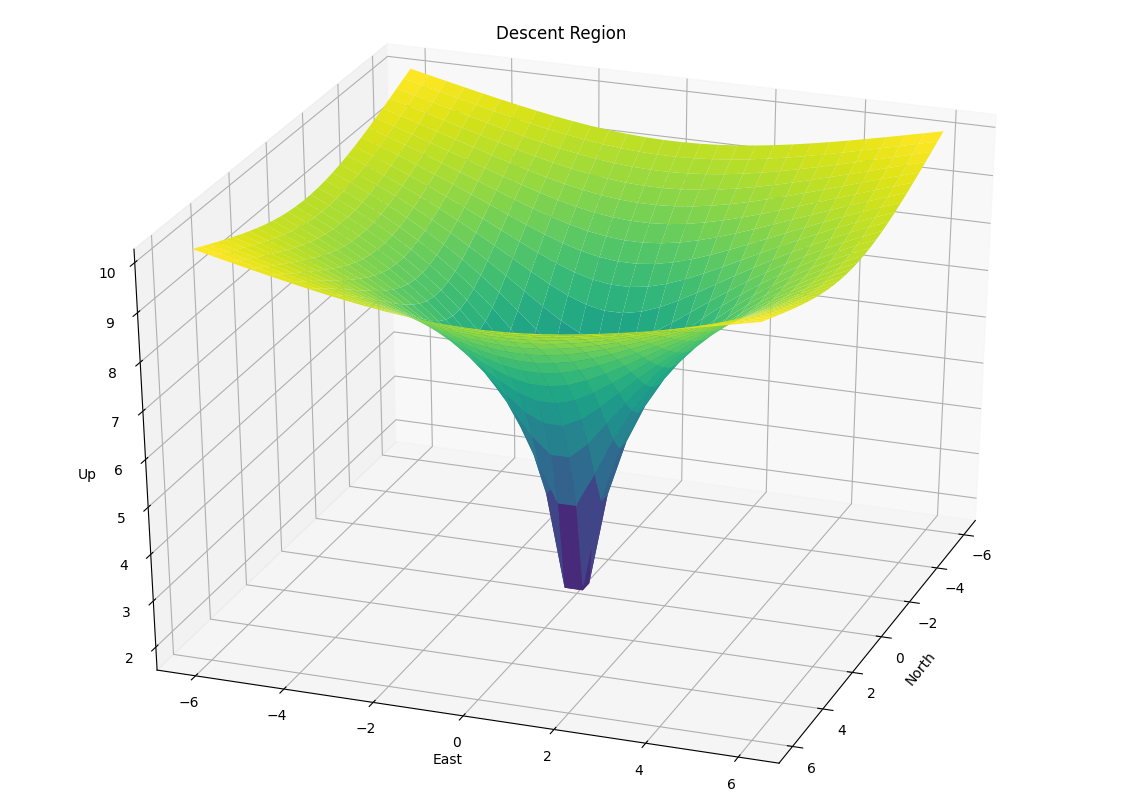
\includegraphics[width=0.75\textwidth]{images/descent_region.png}
    \caption[Example descent region.]{An example descent region for a $k_1=0.15, k_2=0.4$, with the landing platform positioned at $(x,y,z)=(0, 0, 0)$. The drone is allowed to descend in the interior of the plotted surface.}
    \label{fig:descent_region}
\end{figure}

% \begin{etaremune}
%   \item \texttt{NOT\_LANDING}: This is the mode set when the landing controller has been disabled or the landing pad is not yet recognized. Setting this mode triggers a target velocity of 0 in all dimensions, effectively aborting an ongoing landing. This can happen if the user disables the landing or if the landing pad leaves the field of view of the camera for a specified abort time.
%   \item \texttt{APPROACH}: This mode is the first mode set when the landing controller is enabled and the landing pad is located. This mode uses high P-gain, and low D-gain for a quick initial approach, and a 0 I-gain in order not to bias the drone's final velocity.
%   \item \texttt{CLOSE\_APPROACH}: This mode is set once the drone's planar distance to the landing pad is less than some experimentally-determined multiple of the descent distance. The P-gain is lowered and the D-gain is raised in order to gradually slow the drone's approach. The I-gain is still set to 0 at this point. The motivation for this landing phase is to avoid the drone overshooting the landing pad after a quick initial approach.
%   \item \texttt{YAW\_CORRECTION}: During this mode, the drone's yaw PID controller is enabled, which allows the drone to align itself with the landing pad so that the drone's body does not obscure the April Tag marker during final descent. The P-gain of the east and north PID controllers is reduced yet again, and the D-gain increased, in order to avoid overshoot. Descent to some minimum altitude is allowed during this phase, however full descent is not allowed until the drone is aligned within 5 degrees of the landing pad's orientation.
%   \item \texttt{DESCENT}: During this mode, the yaw PID controller is disabled and the heading of the drone is locked by setting its target yaw velocity to 0. Descent below the previously mentioned minimum altitude is allowed. The PID controllers in the north, east, and up directions are still enabled for final velocity correction.
%   \item \texttt{LANDED}: All PID controllers are disabled, east and north target velocities are preserved and continually sent as velocity targets to the drone. The target velocity in the up direction is set to some constant negative value and also sent to the flight controller.
% \end{etaremune}

\begin{table}[h!]
    \centering
    \begin{tabular}{|l|p{12cm}|}
    \hline
        \texttt{NOT\_LANDING} & This is the mode set when the landing controller has been disabled or the landing pad is not yet recognized. Setting this mode triggers a target velocity of 0 in all dimensions, effectively aborting an ongoing landing. This can happen if the user disables the landing or if the landing pad leaves the field of view of the camera for a specified abort time. \\\hline
        \texttt{APPROACH} & This mode is the first mode set when the landing controller is enabled and the landing pad is located. This mode uses high P-gain, and low D-gain for a quick initial approach, and a 0 I-gain in order not to bias the drone's final velocity. \\\hline
        \texttt{CLOSE\_APPROACH} & This mode is set once the drone's planar distance to the landing pad is less than some experimentally-determined multiple of the descent distance. The P-gain is lowered and the D-gain is raised in order to gradually slow the drone's approach. The I-gain is still set to 0 at this point. The motivation for this landing phase is to avoid the drone overshooting the landing pad after a quick initial approach. \\\hline
        \texttt{YAW\_CORRECTION} & During this mode, the drone's yaw PID controller is enabled, which allows the drone to align itself with the landing pad so that the drone's body does not obscure the April Tag marker during final descent. The P-gain of the east and north PID controllers is reduced yet again, and the D-gain increased, in order to avoid overshoot. Descent to some minimum altitude is allowed during this phase, however full descent is not allowed until the drone is aligned within 5 degrees of the landing pad's orientation. \\\hline
        \texttt{DESCENT} & During this mode, the yaw PID controller is disabled and the heading of the drone is locked by setting its target yaw velocity to 0. Descent below the previously mentioned minimum altitude is allowed. The PID controllers in the north, east, and up directions are still enabled for final velocity correction. \\\hline
        \texttt{LANDED} & All PID controllers are disabled, east and north target velocities are preserved and continually sent as velocity targets to the drone. The target velocity in the up direction is set to some constant negative value and also sent to the flight controller. \\\hline
    \end{tabular}
    \caption{Landing Phases}
    \label{tab:landing_phases}
\end{table}

Each of the landing phases is used only to enable and disable PID controllers and change their gains. However there are two other, redundant checks performed at every iteration of the landing controller's loop. First, the yaw of the drone is locked if the drone's yaw is aligned within 5 degrees of the landing pad's yaw orientation. This is done simply by disabling the yaw PID controller and setting a target yaw velocity of 0. Second, if the drone is not in the \texttt{LANDED} phase, a separate check disables descent if the drone is outside of the descent region, and enables it otherwise. This is done by disabling the PID controller for the up direction and setting a target up velocity of 0, and re-enabling the PID controller respectively.

The landing controller is enabled or disabled based on the PWM signal given on a user-defined channel. In this case, channel 11 is used, and a PWM signal on this channel with a duty cycle of more than 50\% enables the landing controller. It is disabled otherwise. This allows manual landing abort and also integration of an autonomous landing into semi-autonomous flights.

At the time of this writing, ArduPilot does not appear to have a feature which allows the sudden disarming of a drone's motors, which would be quite useful after the drone has landed. However, ArduPilot does automatically disarm the motors after it detects that the drone has landed, even when the final velocity is non-zero, and even when non-zero target velocities are set. In order to use ArduPilot without editing it, this fact is leveraged, and the motors are allowed to automatically disarm. It is important that the landing pad maintain a constant velocity until the drone disarms.



% , as shown in Figure \ref{fig:landing_system_architecture}. The first is the \texttt{roscore} module which is necessary within the \gls{ROS} framework and which functions as a base server to facilitate communication among the other \gls{ROS} modules. The data flow is as follows:

% \begin{enumerate}
%     \item The drone-mounted camera provides a raw image of the landing pad's fiducial marker.
%     \item The \texttt{usb\_cam} module provides the raw image from the camera to the rest of the \gls{ROS} modules as a topic.
%     \item The \texttt{whycon\_ros} module analyzes the camera frames and attempts to detect and identify WhyCon markers within the image. If it detects a WhyCon marker, it provides the location and rotation of the marker relative to the camera.
%     \item The \texttt{landing\_controller} module monitors the position of the fiducial marker over time, simultaneously determining the relative velocity. It generates an approach trajectory and communicates this in the MAVlink protocol to the ArduPilot software via the \texttt{mavros} module.
%     \item The \texttt{abort\_controller} module continuously monitors the \gls{IMU} conditions of the drone and the visibility of the fiducial marker in order to determine whether an in-progress landing should be aborted.
%     \item The \texttt{mavros} module provides an interface to allow the \gls{ROS} modules to communicate to the ArduPilot software using the MAVlink communication protocol.
% \end{enumerate}

% \begin{figure}[H]
%     \centering
%     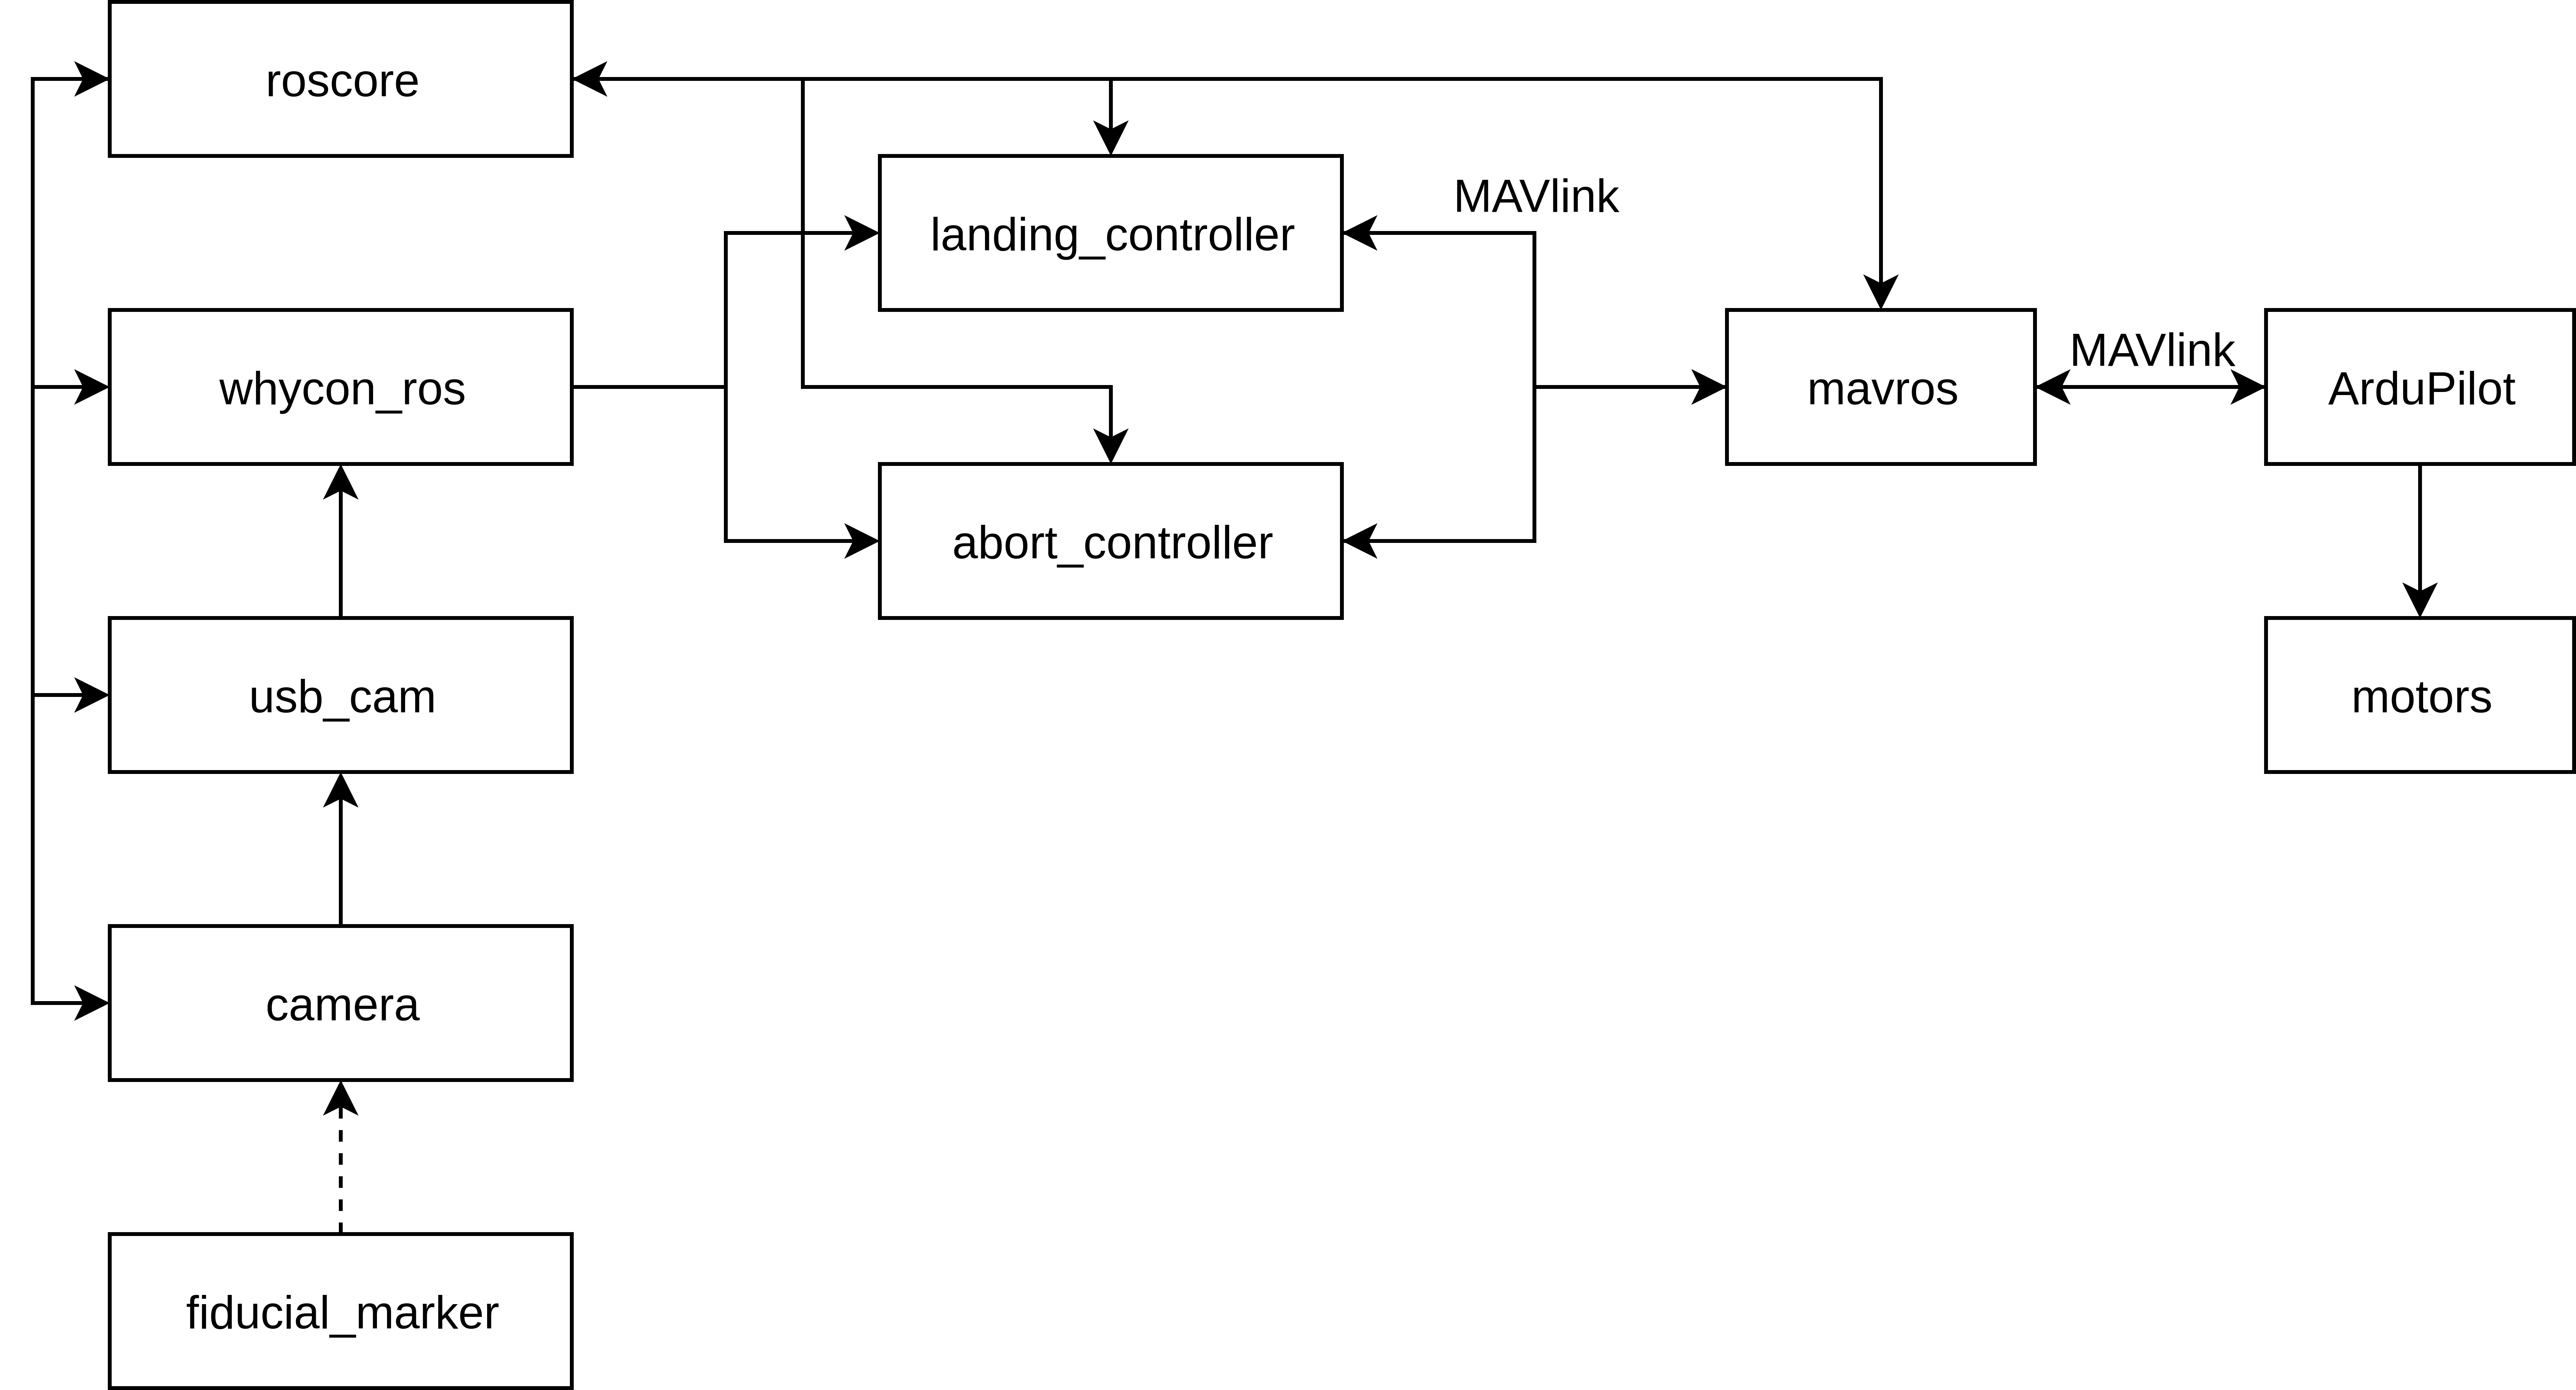
\includegraphics[width=\textwidth]{images/system_architecture.png}
%     \caption{High level landing system architecture.}
%     \label{fig:landing_system_architecture}
% \end{figure}